%%% Folie
\begin{frame}{Leitfragen der heutigen Vorlesung}
    \begin{block}{Allgemeine Hinweise zur Vorlesung}
        \begin{itemize}
            \footnotesize
            \setlength\itemsep{.25em}

            \item Welche Inhalte werden dieses Semester behandelt?
            \item Wie sieht die zeitliche Planung der Vorlesung aus?
            \item Wie sieht die Prüfungsaufgabe dieses Semester aus?
            %\item Welche Hard- und Software wird für die Aufgabe benötigt?
        \end{itemize}
    \end{block}

    \begin{block}{Wiederholung zur IoT-Systemarchitektur}
        \begin{itemize}
            \footnotesize
            \setlength\itemsep{.25em}

            \item Was sind eingebettete Systeme und IoT-Devices?
            \item Was bedeutet der Begriff ,,Industrial Internet of Things''?
            \item Wie sieht eine typische IoT-Architektur im Detail aus?
        \end{itemize}
    \end{block}

    \begin{block}{Systemintegration mit MQTT und Balena}
        \begin{itemize}
            \footnotesize
            \setlength\itemsep{.25em}

            \item Wie kommunizieren IoT-Devices untereinander und mit dem Internet?
            \item Wie funktioniert die asynchrone Kommunikation mit MQTT?
            \item Wie lassen sich IoT-Devices provisionieren und überwachen?
        \end{itemize}
    \end{block}

    \begin{block}{Wiederholung zum Hardwaredesign}
        \begin{itemize}
            \footnotesize
            \setlength\itemsep{.25em}

            \item Welche physikalischen Grundlagen sind für uns relevant?
            \item Wie können Beschädigungen an der Hardware vermieden werden?
            \item Wie lassen sich digitale Ein- und Ausgänge mit dem Pi steuern?
        \end{itemize}
    \end{block}
\end{frame}

%-------------------------------------------------------------------------------
\section{Hinweise zur Vorlesung}
%-------------------------------------------------------------------------------

%%% Folie
\begin{frame}{Kompetenzziele der Vorlesung}
    \begin{itemize}
        \item \textbf{Fachkompetenz:} Die Studierenden kennen den
        \textcolor{NavyBlue}{technischen Aufbau typischer Devices/Embedded Systems}
        im Kontext des Internet of Things. Sie sind in der Lage, entsprechende Devices
        für einen gegebenen Einsatzzweck auszuwählen und zu programmieren.
        \medskip

        \item \textbf{Methodenkompetenz:} Die Studierenden sind in der Lage
        bei der Programmierung von IoT-Geräten systematisch und methodisch vorzugehen.
        \medskip

        \item \textbf{Personale und soziale Kompetenz:} Die Studierenden verstehen die Herausforderungen
        des IoT für Unternehmen, Politik und Gesellschaft und sind in der Lage, diese kompetent zu diskutieren.
        \medskip

        \item \textbf{Übergreifende Handlungskompetenz:} Die Studierenden können reale betriebliche
        Problemstellungen im Kontext von IoT analysieren, \textcolor{NavyBlue}{Konzepte entwerfen}
        und \textcolor{NavyBlue}{IoT-fähige Geräte programmieren} und im Unternehmenskontext integrieren.
        \medskip
    \end{itemize}
\end{frame}

{
\footnotesize
%%% Folie
\begin{frame}{Inhalte der Vorlesung}
        \begin{columns}
            \begin{column}[T]{.5\textwidth}
                \begin{block}{3. Semester}
                    \medskip

                    \begin{enumerate}
                        \item Grundlagen des Internet of Things
                        \item Hardwaredesign für IoT-Anwendungen
                        \item \textcolor{gray}{Praktische Demonstration}
                        \item \textcolor{gray}{Übungsstunde}
                        \item Einführung in Python
                        \item IoT-Entwicklung mit Python
                        \item \textcolor{gray}{Praktische Demonstration}
                        \item \textcolor{gray}{Übungsstunde}
                        \item \textcolor{gray}{Klausurvorbereitung}
                    \end{enumerate}

                    \medskip
                    \textbf{Prüfungsform:} Klausur
                \end{block}
            \end{column}
            \begin{column}[T]{.5\textwidth}
                \begin{block}{4. Semester}
                    \medskip

                    \begin{enumerate}
                        \item Zusammenfassung des dritten Semesters
                        \item Praxisbeispiel zur Python-Programmierung
                        \item Einführung in Docker und die Balena Cloud
                        \item Voraussichtlich: Python Design Patterns
                        \item Voraussichtlich: Embedded Linux
                        \item \textcolor{gray}{Assignment}
                        \item \textcolor{gray}{Assignment}
                        \item \textcolor{gray}{Assignment}
                        \item \textcolor{gray}{Assignment}
                    \end{enumerate}

                    \medskip
                    \textbf{Prüfungsform:} Assignment
                \end{block}
            \end{column}
        \end{columns}
\end{frame}
}

%%% Folie
{
\small

\begin{frame}{Inhalt der Assignment-Prüfung}
    \begin{columns}[onlytextwidth]
        \column[t]{.45\textwidth}
        \begin{block}{Kreativaufgabe}
            \medskip
            \parbox{\linewidth}{
                Ausarbeitung eines Hard- und Softwareentwurfs zu einem vorgegebenen
                IoT-Anwendungsfall.
                \medskip

                Muss die wesentlichen Theorieinhalte beider Semester abdecken.
                Jedoch keinen Quellcode und keine praktische Umsetzung. Nur das Konzept.
            }
        \end{block}

        \column[t]{.45\textwidth}
        \begin{block}{Programmieraufgabe}
            \medskip
            \parbox{\linewidth}{
                Praktische Umsetzung eines vorgegebenen IoT-Anwendungsfalls
                mit dem Raspberry Pi, Python und der Balena Cloud.
                \medskip

                Bewertet werden die Qualität des Quellcodes und die Erfüllung der
                fachlichen Anforderungen.
            }
        \end{block}
    \end{columns}

    \bigskip
    \bigskip
    {
        \normalsize
        Die Aufgabenstellung wird demnächst bereitgestellt.

        \medskip
        Zweimal im Semester werden wir ein \glqq{}Sprint Review\grqq{} zur
        Beurteilung Ihres Fortschritts bei der Programmieraufgabe machen.
    }
\end{frame}
}

%%% Folie
\begin{frame}{Benötigte Hard- und Software}
        \begin{columns}
            \begin{column}[T]{.5\textwidth}
                \textbf{Hardware}
                \medskip

                \parbox{\linewidth}{
                    \footnotesize
                    Kann im WWI-Labor für die Dauer des Moduls kostenlos ausgeliehen
                    werden. Rückgabe am Ende des vierten Semesters, da dieselbe
                    Hardware dann direkt für das IoT-Integrationsseminar und Projekt
                    benötigt wird.
                }
                \medskip

                \begin{itemize}
                    \item Raspberry Pi
                    \item Diverse Sensoren und Aktoren
                \end{itemize}
            \end{column}
            \begin{column}[T]{.5\textwidth}
                \textbf{Software}
                \medskip

                \parbox{\linewidth}{
                    \footnotesize
                    Eigentlich nicht viel. Das meiste ist unter Raspbian bereits
                    installiert oder wird von uns im Laufe der Vorlesung ergänzt.
                    Auf Ihrem Laptop benötigen Sie ggf. noch folgende Programme:
                }
                \medskip

                \begin{itemize}
                    \item Visual Studio Code
                    \item OpenSSH / PuTTY
                    \item Optional: Python
                \end{itemize}
            \end{column}
        \end{columns}
\end{frame}

%%% Folie
{
\small
\setlength{\fboxsep}{0pt}

\begin{frame}{Literaturempfehlungen}
    \begin{columns}
        \column[b]{.33\textwidth}
        \fbox{\includegraphics[height=3.8cm]{img/buch_raspberrypi}}

        \column[b]{.33\textwidth}
        \fbox{\includegraphics[height=3.8cm]{img/buch_practical_electronics}}

        \column[b]{.33\textwidth}
        \fbox{\includegraphics[height=3.8cm]{img/buch_embedded_hardware}}
    \end{columns}

    \vskip 0.6cm

    \begin{columns}
        \column[T]{.5\textwidth}
        \textbf{Raspberry Pi: Das umfassende Handbuch für Maker und Tekkies} \\ Rheinwerk Verlag, 2018

        \column[T]{.5\textwidth}
        \textbf{Practical Electronics for Inventors} \\ McGraw-Hill, 2016
    \end{columns}

    \vskip 0.6cm

    \begin{columns}
        \column[T]{0.5\textwidth}
        \textbf{Designing Embedded Hardware} \\ O'Reilly, 2005
    \end{columns}
\end{frame}
}

%-------------------------------------------------------------------------------
\section{IoT-Systemarchitektur}
%-------------------------------------------------------------------------------

{
\small

%%% Folie
\begin{frame}{Definition ,,Eingebettetes Computersystem''}
    \begin{block}{Definition}
        \parbox{\linewidth}{
            \smallskip

            Eingebettete Systeme sind kleine Mikrocomputer, die innerhalb eines größeren Geräts
            meist unsichtbar verbaut sind, um seine Funktionen zu steuern und überwachen. In vielen
            Fällen geben sie einem Gerät überhaupt erst seine Funktion, ohne dass dies für den
            Anwender offensichtlich ist.
            \smallskip

            Ihre grundsätzliche Architektur ist dieselbe wie bei konventionellen Computern,
            jedoch verfügen sie über weitaus weniger, genau auf den Anwendungsfall zugeschnittene
            Ressourcen bei minimalen Kosten, Platzbedarf und Energieverbrauch. Der Leitgedanke
            hierbei lautet ,,so viel wie gerade nötig, so wenig wie absolut möglich''.
            Eingebettete Systeme sind meist in sich geschlossene Systeme mit deterministischem
            Systemverhalten, die rund um die Uhr laufen und exakt eine Aufgabe erfüllen.
        }
    \end{block}

    \begin{block}{Beispiele}
        \begin{columns}[onlytextwidth]
            \column[b]{.2\textwidth}
            \includegraphics[width=\textwidth]{img/funkwecker}

            \column[b]{.2\textwidth}
            \includegraphics[width=\textwidth]{img/washing-machine-2617514_1280}

            \column[b]{.2\textwidth}
            \includegraphics[width=\textwidth]{img/nes-2649705_1280}

            \column[b]{.2\textwidth}
            \includegraphics[width=\textwidth]{img/keyboards}

            \column[b]{.2\textwidth}
            \includegraphics[width=\textwidth]{img/car-1281640_1280}
        \end{columns}
    \end{block}
\end{frame}

%%% Folie
\begin{frame}{Definition ,,Internet of Things''}
    \begin{block}{Definition}
        \parbox{\linewidth}{
            \smallskip

            IoT-Devices sind eine Teilmenge eingebetteter Systeme größerer Leistungsklasse mit
            permanenter Internetverbindung. Die ursprüngliche Definition aus dem Jahr 1999
            sah die eindeutige, maschinenlesbare Identifikation physischer Objekte anhand von
            RFID-Tags vor. Heute versteht man darunter an einem physischen Objekt angebrachte,
            direkt mit dem Internet verbundene und über ihre IP-Adresse identifizierte Kleinstcomputer,
            da diese inzwischen auf wenigen Quadratzentimetern Platz finden.
            \smallskip

            Im erweiterten Sinne zählen zum ,,Internet of Things'' heute auch Infrastruktur, Cloud-
            und Backendservices, über welche die Devices miteinander verbunden, verwaltet, gesteuert
            und überwacht werden können.
        }
    \end{block}

    \medskip
    
\includegraphics[width=\textwidth]{img/embedded_typen}

    \begin{block}{Beispiele}
        \begin{columns}[onlytextwidth]
            \column[b]{.33\textwidth}
            \includegraphics[width=\textwidth]{img/heart-rate-monitoring-device-1903997_640}

            \column[b]{.33\textwidth}
            \includegraphics[width=\textwidth]{img/blitzer_pulverhausstrasse}

            \column[b]{.33\textwidth}
            \includegraphics[width=\textwidth]{img/winter-681175_640}
        \end{columns}
    \end{block}
\end{frame}
}

%%% Folie
\begin{frame}{Industrielle IoT-Anwendungsfälle}
    \textbf{Smight -- Smart City Light}
    \hfill
    \Href{https://smight.com/}
    \medskip
    \includegraphics[width=0.49\textwidth]{img/smight1}
    \hfill
    \includegraphics[width=0.49\textwidth]{img/smight2}

    \bigskip

    \textbf{Testfeld autonomes Fahren Baden-Württemberg}
    \hfill
    \Href{https://taf-bw.de/}
    \medskip
    \includegraphics[width=\textwidth]{img/karlsruhe}
\end{frame}

%%% Folie
\begin{frame}{Realisierung von IoT-Anwendungsfällen}
    \parbox{\linewidth}{
        \footnotesize

        Der Wunsch, einen Computer zum \textbf{Messen, Steuern und Regeln}
        physikalischer Vorgänge zu nutzen ist fast so alt wie der Computer
        selbst. Die Miniaturisierung der ersten Computer führt bereits früh
        zur Entwicklung eingebetteter Systeme oder der Anpassung vorhandener
        Computersysteme an eingebettete Anwendungsfälle.

        \medskip

        In diesem Sinne hat der Hypebegriff \textbf{\glqq{}Industrie 4.0\grqq{}}
        zwar seine Berechtigung, ist aber nicht in allen Punkten so neuartig,
        wie es einem Glauben gemacht werden soll. (Relativ) neu ist aber, dass
        wir heute zwei Möglichkeiten haben, eingebettete (IoT-)Anwendungen zu
        realisieren:
    }

    \bigskip

    \begin{columns}
        \begin{column}[b]{.5\textwidth}
            \begin{block}{Projektentwicklung}
                \medskip
                %\begin{center}
                    \includegraphics[width=.4\textwidth]{img/sbc-boards}
                %\end{center}

                \medskip
                \parbox{\linewidth}{
                    \footnotesize
                    \textbf{Sehr hohe Integrationstiefe:}
                    Verwendung günstiger Single Board Computer als Komplettsystem
                    inkl. Ökosystem für Programmiersprachen und Hardware-Erweiterungen.
                }
            \end{block}
        \end{column}

        \begin{column}[b]{.5\textwidth}
            \begin{block}{Produktentwicklung}
                \medskip
                %\begin{center}
                    \includegraphics[width=.4\textwidth]{img/microchip}
                %\end{center}

                \medskip

                \parbox{\linewidth}{
                \footnotesize
                    \textbf{Mittlere Integrationstiefe}:
                    Eigenentwicklung eingebetteter Computersysteme auf Basis diskreter
                    Bausteine für Microcontroller, Flash-Speicher, RAM, I/O, …
                }
            \end{block}
        \end{column}
    \end{columns}
\end{frame}


%%% Folie
{
    \setbeamertemplate{background canvas}{
        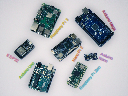
\includegraphics[height=\paperheight, width=\paperwidth]{img/sbc_auswahl}
    }

    \begin{frame}[plain]
    \end{frame}
}

%%% Folie
{
\setbeamertemplate{background canvas}{
    \includegraphics[height=\paperheight, width=\paperwidth]{img/themengebiete1}
}

\begin{frame}[fragile]{IoT -- Ein Haus mit tiefem Keller}
    \only<beamer:2|handout:0>{
        \transdissolve

        \begin{tikzpicture}[remember picture,overlay]
            \node at (5.4cm,0.28cm){
                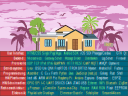
\includegraphics[height=\paperheight, width=\paperwidth]{img/themengebiete4}
            };
        \end{tikzpicture}
    }
\end{frame}
}

%%% Folie
\begin{frame}{Was nutzen wir in der Vorlesung?}
    \begin{center}
        \includegraphics[width=\textwidth]{img/raspi-linux-python}
    \end{center}

    \bigskip

    \parbox{\linewidth}{
        \footnotesize
        Wir nutzen eine Kombination aus \textbf{Raspberry Pi}, \textbf{Linux} und
        \textbf{Python}. Sie ist leistungsstark, leicht zu lernen und in der
        IoT-Entwicklung weit verbreitet.

        \medskip

        \begin{itemize}
            \item \textbf{Rasbperry Pi:} Bietet eine vergleichbare Performance wie
            ein älterer Desktopcomputer.

            \item \textbf{Linux:} Beim mitgelieferten Raspberry Pi OS handelt es
            sich um ein angepasstes Debian-Linux. Die meisten Besonderheiten
            eingebetteter Systeme bleiben verborgen, so dass es fast wie ein
            Desktopsystem nutzbar ist.

            \item \textbf{Python:} Ist eine einsteigerfreundliche Programmiersprache
            mit verschiedenen Anwendungsgebieten. Das Pi in Raspberry Pi stand
            deshalb ursprünglich für \glqq{}Python Interpreter\grqq{}.
        \end{itemize}
    }
\end{frame}

%%% Folie
\begin{frame}{Beispiel einer typischen IoT-Architektur}
    \begin{columns}
        \column{\dimexpr\paperwidth-10pt}
        \includegraphics[width=\textwidth]{img/systemarchitektur}
    \end{columns}
\end{frame}

%%% Folie
{
\scriptsize

\begin{frame}{Aufgabe: Entwurf eines mobilen Datenloggers}
    \begin{block}{Problemstellung}
        \Justified{
            \smallskip
            Der internationale Versand hochwertiger Güter birgt viele Gefahren.
            Raue Umweltbedingungen, falsche Lagerung und unsachgemäße Behandlung
            können schnell zu Beschädigungen führen, deren Zeitpunkt und Ursache
            nachträglich nur schwer nachgewiesen werden kann. Es soll daher ein
            mobiler Datenlogger entworfen werden, der die Waren auf ihrer Reise
            begleitet und kontinuierlich verschiedene Umweltparameter aufzeichnet.
            Die gesammelten Werte sollen auf einer SD-Karte gespeichert und am
            Ende der Reise an einen Server im Internet übertragen werden.
        }
    \end{block}

    \begin{block}{Hardware}
        \smallskip
        Welchen der folgenden Single Board Computer würden Sie verwenden?
        \smallskip

        \begin{columns}
            \column[b]{0.2\textwidth}
            \includegraphics[width=\textwidth]{img/raspberrypi}

            \column[b]{0.2\textwidth}
            \includegraphics[width=\textwidth]{img/arduino}

            \column[b]{0.2\textwidth}
            \includegraphics[width=\textwidth]{img/esp8266}

            \column[b]{0.2\textwidth}
            \includegraphics[width=\textwidth]{img/pi-pico}
        \end{columns}
        \begin{columns}
            \column[b]{0.2\textwidth}
            \textsc{Raspberry Pi 4}

            \column[b]{0.2\textwidth}
            \textsc{Arduino Uno}

            \column[b]{0.2\textwidth}
            \textsc{ESP 8266}

            \column[b]{0.2\textwidth}
            \textsc{Raspberry Pi Pico}
        \end{columns}
    \end{block}

    \begin{block}{Programmierung}
        \begin{itemize}
            \item Welche Programmiersprachen und Frameworks würden Sie verwenden?
            \item Welche Datenbanktechnologie würden Sie im Backend einsetzen?
            \item Wie würden Sie das User Interface realisieren?
        \end{itemize}
    \end{block}
\end{frame}
}


%-------------------------------------------------------------------------------
\section{MQTT und Balena}
%-------------------------------------------------------------------------------

\begin{frame}{Asynchrone Kommunikation mit MQTT}
    \begin{center}
        \includegraphics[width=.9\textwidth]{img/mqtt-beispiel}
    \end{center}

    \bigskip

    \parbox{\linewidth}{
        \scriptsize
        MQTT definiert ein \textcolor{NavyBlue}{asynchrones Kommunikationsprotokoll},
        bei dem \textcolor{NavyBlue}{eine beliebige Anzahl von Sendern} beliebig
        codierte Nachrichten an einen zentralen \textcolor{NavyBlue}{Message Broker}
        senden und dieser die Nachrichten an \textcolor{NavyBlue}{eine beliebige
        Anzahl an Empfängern} weiterleitet. Inhalt und Struktur der Nachrichten
        sind von MQTT nicht vorgegeben, sondern können völlig frei gewählt werden.
        Jedoch muss jede Nachricht an ein sog. \textcolor{NavyBlue}{Topic} gesendet
        werden, damit die Empfänger über einfache Filterregeln entscheiden können,
        welche Nachrichten sie erhalten wollen.
    }
\end{frame}

\begin{frame}{Provisionierung und Deployment mit Balena}
    \begin{columns}
        \column{\dimexpr\paperwidth-4em}
        \includegraphics[width=\textwidth]{img/balena-motivation}
    \end{columns}
\end{frame}

\begin{frame}{Grundprinzip der Balena Cloud}
    \begin{columns}
        \column{\dimexpr\paperwidth-10pt}
        \includegraphics[width=\textwidth]{img/balena-funktionsweise}
    \end{columns}
\end{frame}

\begin{frame}[allowframebreaks]{Deviceseitige Beispielarchitektur}
    \begin{columns}
        \column{\dimexpr\paperwidth-10pt}
        \scriptsize
        \includegraphics[width=\textwidth]{img/balena-beispielarchitektur}

        \medskip
        \url{https://github.com/DennisSchulmeister/dhbwka-wwi-iotws-architektur}
    \end{columns}

    \framebreak
    \begin{columns}
        \column{\dimexpr\paperwidth-10pt}
        \includegraphics[width=\textwidth]{img/balena-grafana}
        \textsc{Grafana Dashboard}
    \end{columns}

    \framebreak
    \begin{columns}
        \column{\dimexpr\paperwidth-10pt}
        \includegraphics[width=\textwidth]{img/balena-webui}
        \textsc{Balena Weboberfläche}
    \end{columns}

    \framebreak
    \begin{columns}
        \column{\dimexpr\paperwidth-10pt}
        \includegraphics[width=\textwidth]{img/balena-cli}
        \textsc{Balena CLI}
    \end{columns}
\end{frame}

\begin{frame}{Benötigte Entwicklungswerkzeuge}
    \begin{columns}
        \column{\dimexpr\paperwidth-10pt}
        \includegraphics[width=\textwidth]{img/balena-werkzeuge}
    \end{columns}
\end{frame}

%-------------------------------------------------------------------------------
\section{Hardwaredesign}
%-------------------------------------------------------------------------------

%%% Folie
\begin{frame}[allowframebreaks]{Was ist elektrischer Strom?}
    \begin{columns}
        \column{\dimexpr\paperwidth-28pt}
        \begin{center}
            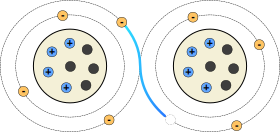
\includegraphics[width=.7\textwidth]{img/atom_elektronenfluss}
        \end{center}
    \end{columns}

    \bigskip

    \parbox{\linewidth}{
        \scriptsize
        Im Normalzustand sind die meisten Atome elektrisch neutral, da sie die
        gleiche Anzahl Protonen wie Elektronen besitzen. Atome mit einem Überschuss
        oder Mangel an Elektronen werden \textbf{Ionen} genannt und sind
        \textbf{elektrisch geladen}. Wurde beispielsweise ein Elektron aus der
        äußeren Hülle eines Atoms heraus gelöst, kann ein benachbartes Elektron
        überspringen, wodurch Strom fließt.
        \smallskip

        \textbf{Elektrischer Strom} entspricht somit der \textbf{Bewegung freier
        Elektronen} innerhalb eines leitfähigen Materials. Strom entsteht daher,
        indem die freien Elektronen durch \textbf{magnetische} oder
        \textbf{chemische Einwirkung} in Bewegung versetzt werden.
        Allerdings darf man das nicht nicht so vorstellen, dass ein Elektron
        geradlinig durch das Material hindurch wandert. Vier mehr nimmt es einen
        zufälligen Weg und schiebt dabei alle anderen Elektronen aus dem Weg,
        da sich Elementarteilchen mit gleicher Ladung immer abstoßen.
    }

    %%% Folie
    \framebreak

    \parbox{\linewidth}{
        \footnotesize
        Folgende Begriffe sind zur Beschreibung elektrischer Ströme von besonderer Bedeutung:
    }

    \begin{block}{Spannung \hfill (Voltage)}
        \smallskip
        \parbox{\linewidth}{
            \scriptsize

            Die Spannung wird immer \textbf{zwischen zwei Punkten} gemessen und beschreibt
            wie viele Elektronen auf der einen Seite zu viel oder auf der anderen Seite zu
            wenig sind. Sie beschreibt somit die \textbf{Ladungsdifferenz} zwischen den beiden
            Punkten und wird in der Einheit \textbf{Volt} gemessen. Sie liefert die Kraft,
            die auf die Elektronen ausgeübt wird, um sie in Bewegung zu setzen und ist
            (sofern die beiden Punkte über ein elektrisch leitendes Material verbunden sind)
            die \textbf{Ursache für den Stromfluss}.
        }
    \end{block}

    \begin{block}{Masse \hfill (Ground)}
        \smallskip
        \parbox{\linewidth}{
            \scriptsize

            Beschreibt in einem Stromkreis den gemeinsamen Bezugspunkt, vom dem aus alle andere
            Spannungen gemessen werden. Entspricht bei einer Batterie meistens dem Minuspol oder
            beim Hausstrom dem Neutralleiter. In einem Stromkreis fließt der Strom gedanklich
            immer vom Pluspol der Stromquelle zur Masse, die meist dem Minuspol der Stromquelle
            entspricht.
        }
    \end{block}

    \begin{block}{Stromstärke \hfill (Current)}
        \smallskip
        \parbox{\linewidth}{
            \scriptsize

            Die Stromstärke gibt an, wie viele Elektronen innerhalb einer gegebenen Zeit einen
            Punkt passieren. Es handelt sich sozusagen um die \textbf{Geschwindigkeit}, mit
            der sich die Elektronen durch den Leiter bewegen. Je mehr Elektronen innerhalb einer
            Zeitspanne durch den Leiter wandern, desto mehr Strom fließt. Die Stromstärke wird
            in der Einheit \textbf{Ampere} gemessen.
        }
    \end{block}

    \begin{block}{Widerstand \hfill (Resistance)}
        \smallskip
        \parbox{\linewidth}{
            \scriptsize

            Jedes Bauteil in einem Stromkreis besitzt einen impliziten Widerstand, der den
            \textbf{Elektronenfluss hindert}, indem ein Teil der Energie in \textbf{Wärme
            oder Strahlung} umgewandelt wird. Ein Widerstand reduziert somit die Stromstärke
            und wird in der Einheit \textbf{Ohm} gemessen. Man kann ihn sich wie einen Knick
            in einem Wasserschlauch vorstellen, durch den nur noch wenig Wasser gelangt,
            obwohl das Wasser mit hohem Druck hinein geschossen wird.
        }
    \end{block}
\end{frame}

\begin{frame}{Schaltpläne zur Dokumentation von Stromkreisen}
    \begin{center}
        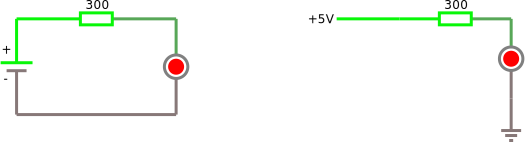
\includegraphics[width=\textwidth]{img/mini-stromkreis}
    \end{center}

    \hfill%
    \CircuitJS{https://www.falstad.com/circuit/circuitjs.html?ctz=CQAgjCAMB0l3BWcMBMcUHYMGZIA4UA2ATmIxAUgoqoQFMBaMMAKADcQ9CAWCwqrr248ooytSqToCFgCdOI4bzCQUQkVVyQWAd2Rq+AkQn5QWYQin3rlq3iapWAJnQBmAQwCuAGwAuDbzoncFEpSFYAJXA1PBAlcAtY+Mk42lCoaTlo7iSRMGxTZJAtc0twAqp4-NMEbl5nNy8-AKCQlJhwlgBzcpq63toMQlCWAA9ObmI40k4EKcorZSsAHQAHMdmIBBRYvAQkBGwIJZAGFiA}
    \bigskip

    \parbox{\linewidth}{
        \scriptsize

        Elektrische Schaltungen werden immer als \textbf{Stromkreis} entworfen
        und in einem \textbf{Schaltplan} dokumentiert. Gedanklich fließt der
        Strom in diesem vom Pluspol zum Minuspol (linke, eher seltene Darstellung)
        bzw. vom Pluspol der Spannungsquelle zur Masse (rechte Darstellung).
        Tatsächlich beruht diese Annahme aber auf einem Irrtum, weil es die
        negativ geladenen Elektronen sind, die sich vom Minus- zum Pluspol bewegen.
        Da sich dadurch aber nur das Vorzeichen in den Berechnungen ändert, wurde
        die Konvention unter dem Namen \textbf{technische Stromrichtung} in Abgrenzung
        zur \textbf{tatsächlichen Stromrichtung} beibehalten.
        \smallskip

        Die Symbole im Schaltplan haben folgende Bedeutung:
        \smallskip

        \begin{center}
            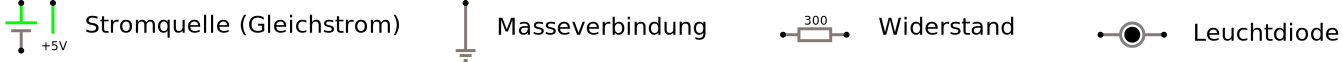
\includegraphics[width=\textwidth]{img/schaltsymbole}
        \end{center}
    }
\end{frame}

%%% Folie
\begin{frame}{Häufig vorkommende Signalarten}
        \begin{columns}
        \column[b]{.5\textwidth}
        \includegraphics[width=\textwidth]{img/strom-analogsensor} \\

        \column[b]{.5\textwidth}
        \includegraphics[width=\textwidth]{img/strom-binary} \\
    \end{columns}

    \bigskip

    \begin{columns}
        \column[b]{.5\textwidth}
        \includegraphics[width=\textwidth]{img/strom-pwm} \\

        \column[b]{.5\textwidth}
        \includegraphics[width=\textwidth]{img/strom-serial} \\
    \end{columns}
\end{frame}

%%% Folie
\begin{frame}{Anschlüsse am Raspberry Pi}
        \begin{center}
            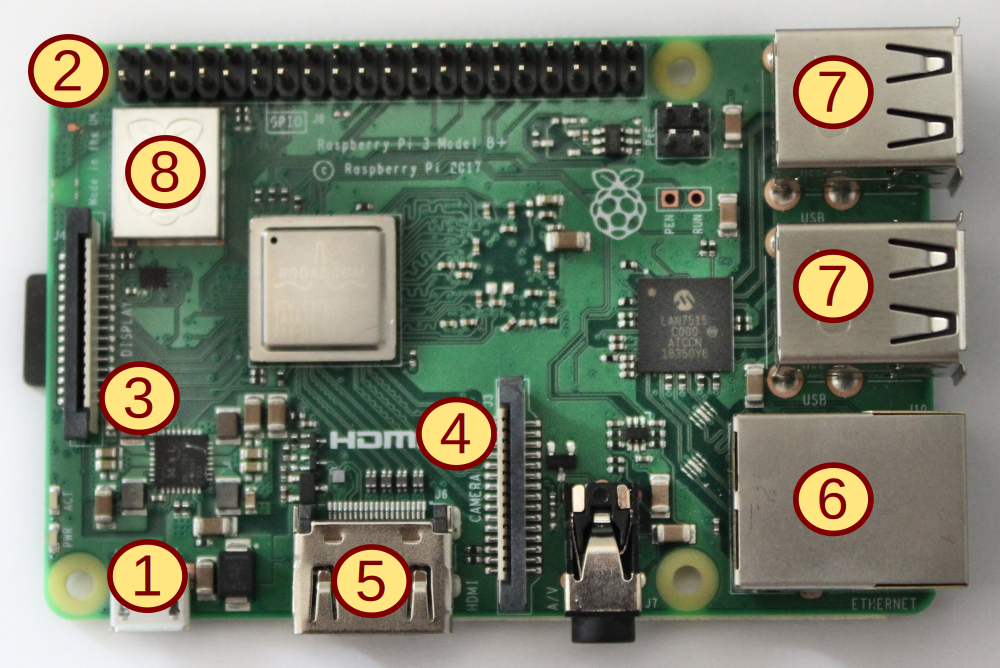
\includegraphics[height=0.5\textheight]{img/raspberry_anschluesse}
        \end{center}

        \smallskip

        \begin{columns}
            \begin{column}[T]{.5\textwidth}
                \begin{enumerate}
                    \item Mini-USB Stromversorgung
                    \item J8 GPIO-Header
                    \item Display Serial Interface
                    \item Camera Serial Interface
                \end{enumerate}
            \end{column}
            \begin{column}[T]{.5\textwidth}
                \begin{enumerate}
                    \setcounter{enumi}{4}   % Zielwert - 1
                    \item HDMI-Bildschirmanschluss
                    \item LAN-Netzwerkanschluss
                    \item USB (4 Stück)
                    \item WiFi, Bluetooth
                \end{enumerate}
            \end{column}
        \end{columns}
\end{frame}

%%% Folie
{
\footnotesize

\begin{frame}{Der J8 GPIO-Header im Detail}
        \begin{columns}
            \column[b]{.5\textwidth}
            \includegraphics[height=.7\textheight]{img/pinout}
            %\includegraphics[width=\textwidth]{img/raspberry_j8}

            \medskip
            \LinkButton{https://pinout.xyz/}{Raspberry Pi Pinout Guide}

            \column[b]{.5\textwidth}
            \begin{block}{Stromquellen}
                \begin{itemize}
                    \item 5V Power
                    \item 3.3V Power
                    \item Ground (Masse)
                \end{itemize}
            \end{block}

            \begin{block}{Digitale Ein-/Ausgänge}
                \begin{itemize}
                    \item GPIO
                    \item Pulsweitenmodulation
                    \item Asynchron serielle Kommunikation
                    \item Synchron serielle Kommunikation \\ (SPI, I²C, I²S, 1-Wire)
                \end{itemize}
            \end{block}

            \begin{alertblock}{Keine analogen Ein-/Ausgänge!}
            \end{alertblock}
        \end{columns}
\end{frame}
}

%%% Folie
{
\footnotesize

\begin{frame}{Bevor es losgehen kann: Maximale Grenzwerte}
    \parbox{\linewidth}{
        Um eine Beschädigung des Raspberry Pi zu vermeiden, müssen folgende Grenzwerte unbedingt
        eingehalten werden. Ggf. müssen daher nach dem Ohmschen Gesetz berechnete Widerstände in
        Serie zu einem Bauteil angeschlossen werden, um die Stromstärke zu begrenzen. Ebenso muss
        die Summe aller zugeführten und entnommenen Ströme betrachtet werden.
    }

    \bigskip
    \renewcommand{\arraystretch}{1.2}

    \begin{tabularx}{\textwidth}{|p{18em}|X|X|}
        \hline
        \textbf{Parameter} & \textbf{Mindestwert} & \textbf{Maximalwert} \\
        \hline

        Betriebsspannung des Pi & 5\,V & 5\,V \\
        \hline

        Stromverbrauch des Pi & 800\,mA (eher mehr) & -- \\
        \hline

        Stromentnahme an den 3.3\,V-Pins & -- & 50\,mA gesamt \\
        \hline

        Stromentnahme an den 5\,V-Pins & -- & 50\,mA gesamt \\
        \hline

        Stromentnahme an einem GPIO-Pin & -- & 16\,mA \\
        \hline

        Stromentnahme an allen GPIO-Pins & -- & 50\,mA gesamt \\
        \hline
    \end{tabularx}

    \bigskip
    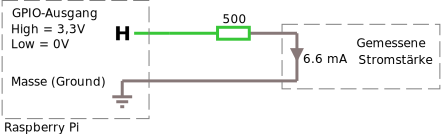
\includegraphics[width=.75\textwidth]{img/stromentnahme-raspi-schaltplan}

    \hfill%
    \CircuitJS{https://www.falstad.com/circuit/circuitjs.html?ctz=CQAgzCAMB0l3BWEBGGAmOaDsWyQBxoBsAnCViApJZdQgKYC0yyAUADIj7JEhr74QWIoP6DqyEADMAhgBsAzvXDQIkVmCzUSAFh18BIXfrBhek6uoDmQkeDO3BYBGihRWAJy48Dg477cqdQAjIRIkNAQkIh0KTX11AHcjPXteYScHdQAPEBiScHwKLDQTEmp9ZFcAJRkFAAdg+g8PAE8AHQUABQBLVlyiBApsVywdCGwkStcAcS6ASQB5RgBBAFcFKxkAOyt+vIReMB1JLCpwVOmQAFk6pU6AChmPAHs17YATAEp9waPICBYZAQPC8K7sF6JTrtACOnUgADVfocAiVRCRJFcABI9KwAC2hcIUYAANGAkblUJATJBXKgxuBIFMULN6ABbegKJTbej7KlHZAFekFMBoVxXADKABdXmyFFKACceADWvNCqEMx30JDQBWwBXUQA}
\end{frame}
}

%%% Folie
\begin{frame}[allowframebreaks]{Das Ohmsche Gesetz}
    \begin{columns}
        \column{.4\textwidth}
        \begin{center}
            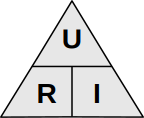
\includegraphics[width=.4\textwidth]{img/formel_uri}
        \end{center}

        \medskip

        \begin{tabular}{ccll}
            $U$ & = & $R \times I$ & {\scriptsize Spannung in Volt} \\
            $R$ & = & $U / I$ & {\scriptsize Widerstand in Ohm} \\
            $I$ & = & $U / R$ & {\scriptsize Stromstärke in Ampere}\\
        \end{tabular}

        \column{0.6\textwidth}
        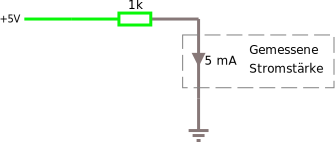
\includegraphics[width=\textwidth]{img/ohmsches-gesetz-schaltplan}

        \hfill%
        \CircuitJS{https://www.falstad.com/circuit/circuitjs.html?ctz=CQAgjCAMB0l3BWcMBMcUHYMGZIA4UA2ATmIxAUgoqoQFMBaMMAKACURiAWLkbQvCDx4q-QVSpdaUGTAQsATpx58ByDClXjkcFtgxUwkDVvWaegiBJYBzMyAv2uI2SwAe4MCmwPIP5sQ+UoQO4JoA4nQAtnQAzrF0AHZ07p7eDiiaASFcKEi8XiAAygAuCgD2UbElACcKANYpAEbICCHYeAVoglz6UCxAA}
    \end{columns}

    \bigskip

    \Justified{
        \scriptsize

        Die \textbf{Spannung} einer Stromquelle sorgt dafür, dass sich die Elektronen in
        Bewegung setzen und ein Strom fließt, wenn zwischen beiden Polen eine elektrische
        Verbindung hergestellt wird. Die dabei entstehende \textbf{Stromstärke} hängt
        vom \textbf{Widerstand} aller durchlaufenen Bauteile (und dem Innenwiderstand
        der Stromquelle) ab. In bestimmten Fällen kann ein linearer Zusammenhang entsprechend
        der Formel $I = U / R$ angenommen werden, so dass mit zwei bekannten Werten
        der dritte errechnet werden kann.
        \smallskip

        Für uns ist dies besonders wichtig, um die maximale Stromstärke zu begrenzen,
        die der Raspberry Pi an ein angeschlossenes Bauteil abgibt, um sowohl den
        Rasbperry Pi als auch das Bauteil vor Beschädigungen zu schützen. Beispiele
        für typische Fragestellungen sind:

        \begin{itemize}
            \item Welche Stromstärke fließt durch eine Schaltung (wie viel Strom ,,zieht`` die Schaltung)?
            \item Welcher Widerstand wird benötigt, um eine bestimmte Stromstärke zu erhalten?
            \item Liegt die Stromstärke innerhalb der erlaubten Grenzen für den Raspberry Pi und das Bauteil?
        \end{itemize}
    }

    \framebreak

    \textcolor{gray}{
        \tiny
        \textbf{Kennlinie:} Stromstärke in Abhängigkeit zur Spannung, der Widerstand entspricht der Tangentensteigung
    }
    {
        \footnotesize

        \begin{columns}
            \column{.33\textwidth}
            \includegraphics[width=\textwidth]{img/kennlinie-widerstand} \\
            \smallskip
            \hfill \textbf{Widerstand} \hfill%
            \raisebox{-0.4\height}{\includegraphics[width=2.5em]{img/komponenten_elementar_widerstand}}


            \column{.33\textwidth}
            \includegraphics[width=\textwidth]{img/kennlinie-diode} \\
            \smallskip
            \hfill \textbf{Leuchtdiode} \hfill%
            \raisebox{-0.4\height}{\includegraphics[width=2.5em]{img/komponenten_elementar_led}}

            \column{.33\textwidth}
            \includegraphics[width=\textwidth]{img/kennlinie-transistor} \\
            \smallskip
            \hfill \textbf{npn-Transistor} \hfill%
            \raisebox{-0.4\height}{\includegraphics[width=2.5em]{img/komponenten_elementar_transistor}}
        \end{columns}
    }
    \bigskip

    \Justified{
        \scriptsize

        Das Ohmsche Gesetz gilt nur für \textbf{ideale Widerstände}, die deshalb auch
        \textbf{ohmsche Widerstände} genannt werden. Genau genommen besagt es, dass
        der Widerstand solcher Bauteile für jede Spannung derselbe ist und sich die
        Stromstärke daher linear zur Spannung verhält. In unserem Fall handelt es sich
        dabei um kleine Keramikwiderstände, die wir in unsere Schaltungen einbauen
        (Abbildung links).
        \smallskip

        Insbesondere Bauteile auf Halbleiterbasis besitzen jedoch eine \textbf{nicht-lineare Kennlinie},
        so dass die durchfließende Stromstärke nicht linear von der Spannung abhängt. Der Widerstand
        dieser Bauteile ergibt sich ebenfalls aus Spannung und Stromstärke, besitzt aber keinen konstanten
        Wert. In Anlehnung an das Ohmsche Gesetz kann er näherungsweise als \textbf{differentieller
        Widerstand} $r = \Delta U / \Delta I$ berechnet werden (sog. Kleinsignalverhalten).
    }
\end{frame}

%%% Folie
{
\scriptsize

\begin{frame}{Binärsignal ausgeben am Beispiel einer LED}
    \Justified{
        Jeder \textbf{GPIO-Pin} kann softwaregesteuert als \textbf{Eingang oder Ausgang} konfiguriert
        werden. Ausgangspins stellen eine Spannung von \textbf{ca. 3,3\,V} zur Verfügung, um eine
        logische Eins zu signalisieren, sowie \textbf{0\,V} (entspricht einer Verbindung gegen Masse)
        für eine logische Null.
        \smallskip

        Der entnommene Strom muss in der Regel durch einen \textbf{Widerstand} begrenzt werden.
        Da die verfügbare Spannung und die gewünschte Stromstärke bekannt sind, kann dieser mit
        dem \textbf{Ohmschen Gesetz} leicht berechnet werden. Dabei muss jedoch auch der innere
        Widerstand des angeschlossenen Bauteils, der nicht immer leicht zu ermitteln ist,
        berücksichtigt werden, da dieser den Gesamtwiderstand erhöht und die Strommenge dadurch
        zusätzlich begrenzt.
        \smallskip

        \textcolor{red}{
            Die entnommenen Ströme dürfen nicht größer als 16\,mA und ihre Summe nicht größer als 50\,mA sein.
        }
    }

    \bigskip

    \begin{columns}
        \column{0.5\textwidth}
        \includegraphics[width=\textwidth]{img/led_direkt_circuitjs}
        \smallskip

        \CircuitJS{https://www.falstad.com/circuit/circuitjs.html?ctz=CQAgjCAMB0l3BWcMBMcUHYMGZIA4UA2ATmIxAUgoqoQFMBaMMAKAHMRCUAWCsFTjwoo8UKCwBOnDAO7dRGQqLmiq2XCzBcQi5fJB5ss-QIAmdAGYBDAK4AbAC4M7dU+DFUYkVgBlpx0S5eFTEIazsAZzoQbGhscT9CGRi8XiCU3iowq0jo2PjISX8MnSUStQ1sDCpDAWxUkGJ+EohPFiqaoxAQpoD3NoB3Rub63l7u-UKh8Z7mhGbCrQFdEtqSs0tbR2dXfo9YVmm55vT5gULE5KMqdOvQkHComLjxKSS6tFLRO4qpr5jPmsfu1qgYundxndWuIjh8qJCGoUAEacBCEECYJDcDDECho8QAD26igoeFo81J8V4zQASlYIgAHJF0CQSACeAB0IgAFACWLCJlG+QgQxF4RnI1IEAHFuQBJADyDAAgjYImwrAA7NgCmiieZpSACeaS8ACACy9KiXIAFNKJAB7Gya0wASl1lHI9XRovi9VxUpAssVKrVGu1Hsgkopvu6CGCZqD8qVqvVWp1KLWmAExHqePIhSJqVoeCQTRLykT0roAFs6BEopq6LrDLjCJB0U025AA4mAMoOR01iIOAAnEgA1nRNSwgA}

        \column{0.5\textwidth}
        \includegraphics[width=\textwidth]{img/led_direkt_foto}
    \end{columns}
\end{frame}
}

%%% Folie
{
\scriptsize

\begin{frame}{Große Lasten über Relais schalten}
    \Justified{
        Große Lasten können aus Sicherheitsgründen nur mechanisch geschaltet werden.
        Der Hardwareaufbau gliedert sich dann ein einen \textbf{Steuerstromkreis} und
        einen \textbf{Arbeitsstromkreis}, die komplett \textbf{galvanisch Entkoppelt}
        sind und deshalb jeweils eigene Stromquellen besitzen.
        Ein \textbf{Relais} dient als ferngesteuerter Schalter, der den Arbeitsstromkreis
        unterbrechen und schließen kann. Im Inneren besteht es aus einem durch den
        Steuerstromkreis gespeisten Elektromagneten und einem magnetischen Kippschalter.
        Beim Umschalten entsteht das charakteristische Klickgeräusch.
    }

    \medskip

    \begin{columns}
        \column{0.6\textwidth}
        \includegraphics[width=.9\textwidth]{img/led_relais_circuitjs}
        \smallskip

        \CircuitJS{https://www.falstad.com/circuit/circuitjs.html?ctz=CQAgjCAMB0l3BWcMBMcUHYMGZIA4UA2ATmIxAUgoqoQFMBaMMAKABkQ9jCQAWMHnl54+AqOBAAzAIYAbAM50Q2aNigsA5p2F9u2kQjApxkFgCdOe-jzI9r4zKYBGnPFWxCQGSLwq81pgAeXpDGCAjEXlgUhMa+RiAAStLyAA5OdGZmAJ4AOvIACgCWLMEYaHwVbnYoavHGAOIFAJIA8gwAggCu8hrSAHYapV5gkZRUeGBqlHXgxgCyKYr5ABQNZgD2Xf0AJgCULGAYIrbKnmD4Ih6+PBCoULDM2BjE2BfYvMKYvITkMJBIC7wOAPSAQCr-HyggHgFgAd3ARio9mYFV4elMCNRyL0QhE6J4QWQFUMtyMYVGfDmIAAygAXOhdTLyOmbAC2AGszHQivJDpNLDwUAhbqFfMLCeBiCheLAhIZuJQpngeJRqf9fBr4YiKhKdciQZjkHh8SDsXxDdrzSjLqJCcMLmARDK1Ki1DK7NSOmYMkU6fIWeyuTy+Vo8cooeHsBD1Aio1DTrhNdrEwmMDxrupEoKQHrw3qqAb1SZoAgrWLcyL9ZX7S4TVQ0CJvGoPsmypBXcQRHgEOQ0BB6iAAKKBBlmfp0fL09kAN2ZGzMGm2QyAA}

        \column{0.4\textwidth}
        \includegraphics[width=\textwidth]{img/led_relais_foto}
    \end{columns}
\end{frame}
}

%%% Folie
{
\scriptsize

\begin{frame}{Digitaleingang mit Active-High-Logik (z.B. Taster)}
    \Justified{
        Viele Sensoren stellen lediglich einen \textbf{Kontakt zwischen zwei Pins} her, wenn ein bestimmtes
        Ereignis eintritt, zum Beispiel wenn ein Schalter gedrückt, eine Berührung mit einem Hindernis
        oder ein Feuer erkannt wird. Indem man einen Pin des Sensors mit einer 3,3\,V Versorgungsspannung
        und den anderen Pin mit einem GPIO-Eingang verbindet, lässt sich eine sog. \textbf{Active-High-Logik}
        realisieren. Dies bedeutet, dass der GPIO-Eingang durch den Sensor mit 3,3\,V gespeist wird,
        wenn das Ereignis eintritt, was vom Raspberry Pi als logische Eins interpretiert wird.
        \smallskip

        Jedoch sollte in diesem Fall immer der \textbf{interne Pull-Down-Widerstand} des Raspberry Pi
        aktiviert werden, um den Eingang auf Masse zu ziehen, wenn kein Signal anliegt. Andernfalls
        führen \textbf{parasitäre Induktionen} zu zufälligen Phantomwerten und Fehlmessungen.
        \medskip
    }

    \begin{columns}
        \column{0.6\textwidth}
        \includegraphics[width=\textwidth]{img/button_pulldown_circuitjs}
        \bigskip

        \CircuitJS{https://www.falstad.com/circuit/circuitjs.html?ctz=CQAgjCAMB0l3BWcMBMcUHYMGZIA4UA2ATmIxAUgoqoQFMBaMMAKAFkQ9sUQAWPKjkJ8BUECmgIWADxCEUPXhl4gMkFUvIqwPAOIAFAJIB5BgFEAlgDsA5gENbLAM4hiOkVVKLRVCADM7ABsnOhYAJU5uPjhVbGFeGKoqBJBsaGwxJMkWG1jhBEJBOIoMYSSWAHc8ikLVPBUC8oAnOo1RDHqapJp4GTkFPmIVEmSyPnAeAEEAYwAXCwA3OgAdJwAJCxsACz75HgKMjDB8wniJkDY7JxDVgApdJoB7AFcrABMASkrXYm9PX+i5SqXkBkUUiRYLS4f1c7n43TAvVkeE68gyiLASHkZ3c+megUCDAAIo8KlYGAB1CxvOhNJyzBxvPpucgIDDEZB4DkIAjjdwAIToNiadCsAC9XjZVjSmqsAMqzJ4AW3pABOmgBrUKyNzcwgQDG0Qgac5UmX0xmrCVNFi8FAZYjFBC8FQoxRDKC2+2cYhUQpIAR4CjYFSQFgAIzBqUIQcKsfwntk8iDCQgpw06j5PH0pNpu2Y-WGeGE8i05zCVwADuHaU0AJ6rfQWFhAA}

        \column{0.4\textwidth}
        \includegraphics[width=\textwidth]{img/button_pulldown_foto}
    \end{columns}
\end{frame}
}

%%% Folie
{
\scriptsize

\begin{frame}{Digitaleingang mit Active-Low-Logik (z.B. Lichtschranke)}
    \Justified{
        Einige Sensoren \textbf{unterbrechen einen Kontakt}, wenn die festzustellende
        Bedingung eintritt. Dies trifft zum Beispiel auf Lichtschranken zu, die an ihrem
        Ausgang so lange einen Strom liefern, bis sie unterbrochen werden. Da man in der
        Regel aber genau die Unterbrechungen zählen will, würde dies eine entsprechende
        \textbf{Sonderbehandlung zur Invertierung der Messwerte in der Software} erforderlich
        machen. Einfacher und sicherer ist stattdessen, das Sensorsignal mit einer
        \textbf{Active-Low-Logik} bereits im Hardwareaufbau zu negieren.
        \smallskip

        Indem der interne Pull-Up-Widerstand des Raspberry Pi aktiviert wird, wird der GPIO-Eingang bei
        einer Unterbrechung des Eingangssignals auf eine logische Eins hochgezogen. Die meiste Zeit kann
        der Strom jedoch über den Sensor nach Masse abfließen, so dass der Raspberry Pi stattdessen eine
        logische Null sieht.
    }

    \bigskip

    \begin{columns}
        \column{0.6\textwidth}
        \includegraphics[width=\textwidth]{img/button_pullup_circuitjs}
        \bigskip

        \CircuitJS{https://www.falstad.com/circuit/circuitjs.html?ctz=CQAgjCAMB0l3BWcMBMcUHYMGZIA4UA2ATmIxAUgoqoQFMBaMMAKAFkQM8AWEbvKjkJ8BUECmgIWADxCEUKPhl4ZIvblj7hFAcQAKASQDyDAKIBLAHYBzAIY2WAZxDEwi-lVLvRVCADNbABtHOhYAJU4ePjhObGFuGKoqBJBsaGwxJMkWa1jhBEJBOIoMYSSWAHc8ikLI3gLygCc66MEojzFKeBk5BT5iXkI8eLItNxAAQQBjABdzADc6AB1HABkAewqe+UUCjIwwfMJ47RA2W0cQlYAKHUb1gFdLABMASkqXYl3arnrayB6wwy2GISDI5BBeDGij0D0CgQYAFUAA4MADq5medEajhm9meLG4KAyw2I0QgeDAZO4RKgLAARiA8NhFHEoYV2fg6bJ5FCEhBjuo1NCQHpNtjtsxeoNhr1yLxxmELsj6djGgBPFZ6cwfVzeNrqHwsZpeESeL41JKpXA9Yh4JCEXDIUpybAZBWKDFYnF4l4rABeD0atqihG4ZOYBTkCHcpwAQnRrI06JZAzYVt6VgBlGb3AC2uIAJ40ANahIkZMCQFBkwhgJBVsDkBApAFAA}

        \column{0.4\textwidth}
        \includegraphics[width=\textwidth]{img/button_pullup_foto}
    \end{columns}
\end{frame}
}

%%% Folie
{
\scriptsize

\begin{frame}{Praxisbeispiele}
    \begin{block}{R2R-Kette zur Erzeugung von Analogsignalen}
        \bigskip

        \begin{columns}
            \column{0.5\textwidth}
            \includegraphics[width=\textwidth]{img/r2r-dac}
            \bigskip

            \column{0.5\textwidth}
            \Justified{
                Mit einer Kette von Widerständen lässt sich ein einfacher Analogwandler
                zur Erzeugung variabler Spannungen aufbauen. Benannt ist das Prinzip nach
                den Widerstandswerten $R$ und $2R$, da diese zusammen einen Spannungsteiler
                bilden, durch den verschieden große Teilspannungen aufsummiert werden.
            }

            \bigskip
            \CircuitJS{https://www.falstad.com/circuit/circuitjs.html?ctz=CQAgjCAMB0l3BWcMBMcUHYMGZIA4UA2ATmIxEIBYQkFIaBTAWjDACgAZcQ+sS6sD3AZCUMQDMAhgBsAzgxpROIFJV78Va4aPr0pchUkjLsacBtO8RYvTPmLjAJ27qBQvLuTwnm175AeYmDePpbm1GGBvCFszoL0gaoJnnTwsf6BkSne6VkgaslBMQDm+XAB9AXgYCg2bADyFU2CzeDp8U2BUTQ5zl2FfNTROVyBg83Wnvr2RmxAA}
        \end{columns}
    \end{block}

    \vfill

    \begin{block}{Scan-Matrix zum Auslesen vieler Schalter}
        \bigskip
        \begin{columns}
            \column{0.5\textwidth}
            \includegraphics[width=.9\textwidth]{img/keyscanmatrix}
            \bigskip

            \column{0.5\textwidth}
            \Justified{
                GPIO-Pins hat man in der Regel immer zu wenig. Vor allem, wenn jedes
                Bauteil direkt mit einem Pin verbunden wird. Mit einer Reihe von Dioden
                und etwas geschickter Programmierung kann dem oft entgegen gewirkt werden.
                Das Beispiel zeigt den Aufbau einer einfachen Scan-Matrix, bei der der
                Microcontroller in schneller Abfolge immer eine Zeile und eine Reihe von
                Schaltern überprüft.
            }

            \bigskip
            \CircuitJS{https://www.falstad.com/circuit/circuitjs.html?ctz=CQAgjCAMB0l3BWcMBMcUHYMGZIA4UA2ATmIxAUgoqoQFMBaMMAKAGcRC88QVuQMXXvypUAZgEMANmzrtO-bEME8lPKhEky5HLjwAs+nipCH14EFtny8hfcJ7FDDqBas6Qt+2pBPvQ0Utpaw4vUyNfZzNXTWCPMEh9Kj4eZjQXDSDteQSkkB80qh9M9xzEqmjC8PNxOJYAEwEhFKbVdJQQerpJAFcpABcG1vzlISTkzu6JPsHGk2j5vAmu3oGhvxcN7HbJ1dnI-0couF5d6bXGjeirpdOV8-2qlqrt5amZoZehKvG794vwGB0pUgRVbh17h8AO6A9KvA75dKQFgwrbpEzw5EwjHpQj4RGiFGwionK4nLEI37zclE6lUPEGGkwn63G6E1FRW6LdnDIz0-F8qBEvQuEXFYWKIQi6IUsItMLimEKoRhGVE3LJfgakbqdXlHXIPJqgAyCh4LRFKBQ9kC7moyNNcv4cutrlq2ntLFN2ue+qtNrccU9AA8FEgwDhPBgOhHCKZePYAOIABQAkgB5BgAQR6bAA5gATgB2ebkoa49jApGQkGwvEgHUrcYAyv06D06AAnIsAGgAOmwoXQpABjAAWdAHzYADtI2wPpvnh3RZEWB1CAJad+osACynHx8IQzkxvGgCD3B8ZtGOgRQ58vDNMt2P9kFyQfodfFGwSGj9gQbADATEAUwzBgAFENxLYtSxYL99A6BBCCQbg42Q4CwDjY0N26Ls1zYLoCNbCR+lzAcujYAcACs6CHDcpA3UtiPHOcuzYFggA}
        \end{columns}
    \end{block}
\end{frame}
}

%%% Folie
\begin{frame}{Aufgabe: Fragen zur Vertiefung}
    \begin{block}{Spannung und Stromstärke}
        \smallskip
        \begin{enumerate}
            \item Eine typische Steckdose liefert 230\,V und kann maximal mit
            16\,A belastet werden. Was bedeuten diese beiden Zahlen?

            \item Was ist der Unterschied zwischen Gleichstrom und Wechselstrom?
        \end{enumerate}
    \end{block}

    \begin{block}{Anwendung des Ohmschen Gesetzes}
        \smallskip
        \begin{enumerate}
            \setcounter{enumi}{3}

            \item Wie kann die Stromentnahme an einem GPIO-Pin des Raspberry Pi
            auf maximal 10\,mA begrenzt werden?

            \item Was sind die E-Serien für Widerstände?
        \end{enumerate}
    \end{block}

    \begin{block}{Weitere Hardwarebauteile}
        \smallskip
        \begin{enumerate}
            \setcounter{enumi}{5}

            \item Wie funktioniert Motor Driver in Form einer H-Brücke und wie
            lassen sich damit Richtung und Geschwindigkeit eines Motors regeln?
        \end{enumerate}
    \end{block}
\end{frame}
